%%% Esqueleto base de la presentacion
%%% No agregar las paginas con un include
%%% Lo que quieran aportar deben ser usuarios del TRAC

\documentclass{beamer}
\usepackage[spanish,activeacute]{babel}
\usepackage[utf8]{inputenc}
\usepackage{listings}
\usepackage{color}
\usepackage{graphics}
\definecolor{gray2}{rgb}{100,100,100}

\usetheme[pageofpages=of,% String used between the current page and the
                         % total page count.
          alternativetitlepage=true,% Use the fancy title page.
          titlepagelogo=img/logo,% Logo for the first page.
          watermark=img/di-off,% Watermark used in every page.
          watermarkheight=100px,% Height of the watermark.
          watermarkheightmult=4,% The watermark image is 4 times bigger
                                % than watermarkheight.
          ]{Torino}

\usecolortheme{nouvelle}

\author{\normalsize
\textbf{Integrantes:}\\
Cristian Maureira\\
Rodrigo Fernández\\
Ignacio Villacura\\
Gabriel Zamora\\
\vspace{0.2cm}
\textbf{Jefe de Proyecto:}\\
Esteban Bombal\\
\textcolor{gray}{ebombal@alumnos.inf.utfsm.cl}
}
\title{\Huge Control de Acceso Lógico}
\subtitle{\Large \textit{``Propuesta de Proyecto''}}
\institute{Universidad Técnica Federico Santa María}
%\date{\today}

\begin{document}
\begin{frame}[t,plain]
\titlepage
\end{frame}


\section{Resumen}

\frame{
\frametitle{Resumen}

Implementación de un framework de seguridad basado en Java, llamado \textbf{JAAS}. 
Establecer una conexión a servicios de directorios mediante \textbf{LDAP} para la conexión a la máquina \textbf{JBoss} correspondiente.

}

\section{Formulación general del proyecto}
\frame{
\frametitle{Definición del Problema}
	Posible preturbación entre dos entidades que establecen comunicación

	\begin{figure}[htp]
		\centering
		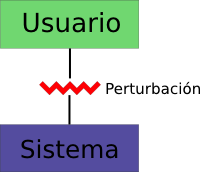
\includegraphics[scale=0.3]{img/user-sist}
		\caption{Comunicación Usuario-Sistema y sus perturbaciones}
		\label{fig:fig1}
	\end{figure}
}

\frame{
\frametitle{Objetivos del Proyecto}
	El objetivo principal de nuestro proyecto es:
\begin{itemize}
\item Implementar el modelo API de autenticación JAAS (Java Authentication and Authorization Service) para controlar el acceso, vía autenticación, a máquinas JBoss. 
\end{itemize}
	Nuestros objetivos específicos son:
\begin{itemize}
\item Poder comunicarse con un Servidor de Directorios, como LDAP, o utilizar una base de datos para almacenar la información de los usuarios.
\item Utilizar JAAS, para autentificar vía  web a los usuarios que quieran ingresar a la máquina JBoss.
\item Dar acceso diferenciado a los usuarios, ya sean administrador o usuarios, para poder utilizar la maquina JBoss.
\end{itemize}
}

\frame{	
\frametitle{Resultados Esperados}	

\begin{itemize}
\item Implementar un sistema de autenticación JAAS, de manera
óptima para poder realizar las tareas de comunicación con un Sistema de Directorios, como LDAP, y
permitir la autenticación diferenciada en el ingreso a la máquina JBoss. Esperamos comprender el sistema a fondo, utilizando las correctas
directrices de seguridad que éste posee y dar un servicio óptimo de autenticación de usuarios para los
demás grupos que utilicen el sistema.
	
\item Probar la implementación de JAAS en otros servicios de autenticación como Pam, a través del puente que proporciona JPam y comparar
las ventajas y desventajas que estos dos sistemas poseen y ver como a su vez se puedan ver
complementados.
\end{itemize}

}

\newpage

\section{Planificación del Proyecto}

\frame{
\frametitle{Metodología de Trabajo}
\begin{itemize}
	\item Horarios Semanales de trabajo
	\item Reuniones presenciales
	\item Coordinación y asignación de metas semanales
	\item Worklogs
\end{itemize}
}

\frame{
\frametitle{Plan de Trabajo}

Investigación
\begin{itemize}
	\item JBOSS
	\item Documentación Básica
	\item Uso y aplicación de JAAS en JBOSS
	\item JAAS 
	\item Documentación Básica
	\item Distintos tipos de Uso
	\item Funcionamiento Cliente-Servidor
	\item Sign-On
	\item Políticas de Seguridad
	\item LDAP
	\item Integración LDAP con JAAS
\end{itemize}
}

\frame{
\frametitle{Plan de Trabajo}

Implementación
\begin{itemize}
	\item Implementación simple de plataforma JBOSS 
	\item Implementación simple de protocolo LDAP 
	\item Implementación de Single Sign-On en JAAS 
	\item Implementación de servicio JAAS 
	\item Desarrollo y uso de JAAS en JBOSS usando LDAP 
	\item Desarrolo servicio web sobre JBOSS 
	\item Integración de JAAS y LDAP 
	\item Integración de servicio web y JAAS 
	\item Testing y Debugging 
\end{itemize}
}

\frame{
\frametitle{Plan de Trabajo}

Integración entre proyectos 
\begin{itemize}
	\item Integración con proyecto LDAP 
	\item Integración con proyecto JBOSS 
\end{itemize}

}

\frame{
\frametitle{Recursos}

\begin{itemize}
\item Alias de Correo, Trac y Skype
\item Deesarrollo sobre plataforma Linux.
\item  Java Platform, Enterprise Edition (JEE).
\item LDAP, Git, LaTeX, Vi IMproved (VIM) y Planner
\item Hardware a utilizar: 1 servidor del LabIT o LabSD para poder llevar a cabo las pruebas
del proyecto.
\end{itemize}
}

\newpage
\end{document}
